%!TEX TS-program = XeLaTeX
%!TEX TS-program = XeLaTeX
\documentclass[11pt]{article}

\usepackage{amssymb}
\usepackage{amsthm}
\usepackage{amsmath}
\usepackage{mathtools}

\usepackage{fancyhdr}
\usepackage{graphicx}
\usepackage[top=3cm, left=2cm, right=2cm, headheight = 90pt]{geometry}
\usepackage{xltxtra}
\usepackage[font=small,labelfont=bf]{caption}

\usepackage{multicol}

\renewcommand{\theenumi}{\alph{enumi}}


\def\leq{\leqslant}
\def\geq{\geqslant}
\def\N{\mathbb N}
\def\R{\mathbb R}
\def\Z{\mathbb Z}
\DeclarePairedDelimiter\set\{\}

\def\prob{}

\theoremstyle{definition}
\newtheorem{problem}{\prob}


\pagestyle{fancy}

%!TEX TS-program = XeLaTeX

\fancyfoot[CE,CO]{}  % this is to remove page numbers (as you might want for single page docs)

%%!TEX TS-program = XeLaTeX
\renewcommand{\figurename}{Attēls}

\fancyhead[C]{{\Large\bf Pigeonhole 2 - Solutions}\\ \date}

\renewcommand{\theenumi}{\alph{enumi}}


\renewcommand\thesubfigure{(\alph{subfigure})} % see subcaption doc


\begin{document}
%\thispagestyle{fancy}
\noindent 
%\emph{\notes}

%1
\begin{problem}
\textit{[Naval Warfare]} 
Battlefield is a $10 \times 10$ squares grid and Admiral needs to position following ships on this grid: one carrier - rectangle of $1 \times 4$ grid squares; two battleships $1\times3$; three cruisers $1\times2$; and four frigates $1\times1$. Ships have to match cells on grid, they may not touch each other, but are allowed to touch sides of the grid. Prove that
\begin{enumerate}
\item If Admiral starts with larger ships and proceeds to smaller, it can always be done
\item If Admiral starts with some smaller ships, before placing larger ones, it can happen that she can not place all the ships on the battlefield
\end{enumerate}

\textbf{Solution}

In the second case it is possible to arrive at an example (see Figure \ref{fig:shipsStuck})

\begin{center}
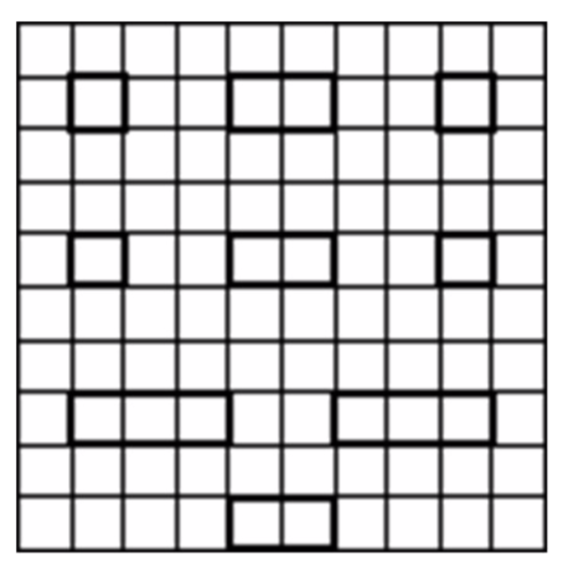
\includegraphics[width=5cm]{StuckShips.png}
\captionof{figure}{Nowhere to put carrier!}
\label{fig:shipsStuck}
\end{center}


For the first part of the problem it is important to note that it is not enough that we will always be able to deploy the last ship - it can happen that we would be able to deploy the last one, but not one of the previous (bigger) ones!

Nevertheless it could be beneficial to reason from this direction. How would we prove that all the frigates can be deployed? We can visualise $16$ locations like this:

\begin{center}
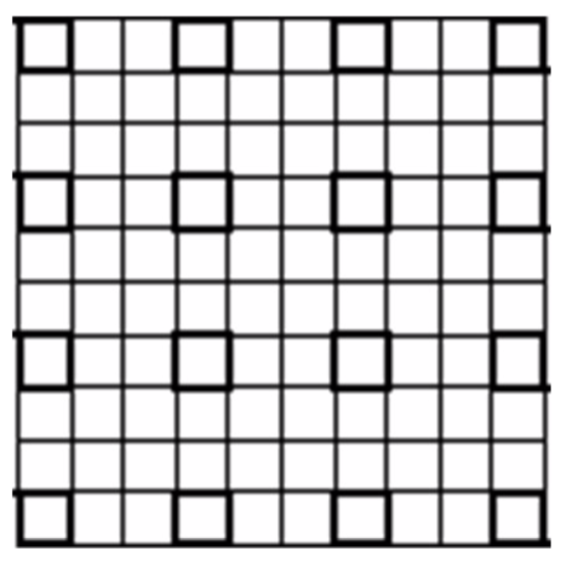
\includegraphics[width=5cm]{SpotForFrigate.png}
\captionof{figure}{Grid for Frigate}
\label{fig:SpotForFrigate}
\end{center}

These marked location have a property that any deployed ship can touch no more than $2$ of these locations and any deployed frigate can touch no more than $1$ of these locations. 
Since the maximum we have deployed so far is $3$ frigates plus $6$ larger ships, no more than $3+6\times 2= 15$ locations are touched. 
Therefore we can deploy a frigate in the untouched location!

Now, working backwards, we also need to prove that it is possible to deploy all the cruisers and all the battleships. We do it with a very similar argument (sans frigate exception) with 
locations seen in Figure \ref{cruiser} and \ref{battleship}



\begin{figure}
\begin{center}
\captionsetup{singlelinecheck=off}
\captionsetup[subfigure]{singlelinecheck=on}
%
%\captionbox{Foo\label{fig:1}}[0.42\textwidth][l]{%
%   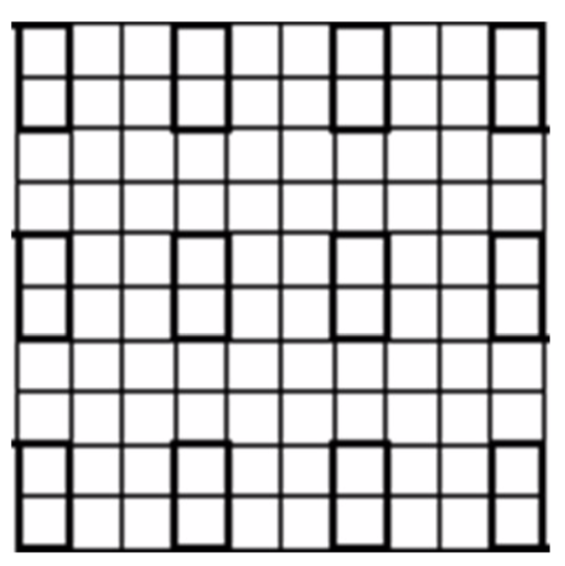
\includegraphics[width=0.20\textwidth]{PlaceForCruiser.png}%
%   \phantomsubcaption\label{fig:1a}% Bug: Produces an unwanted space
%   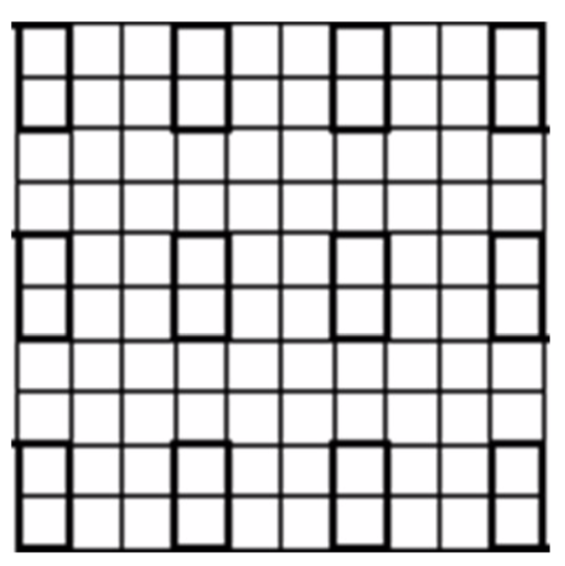
\includegraphics[width=0.20\textwidth]{PlaceForCruiser.png}%
%   \phantomsubcaption\label{fig:1b}%
%\\
%   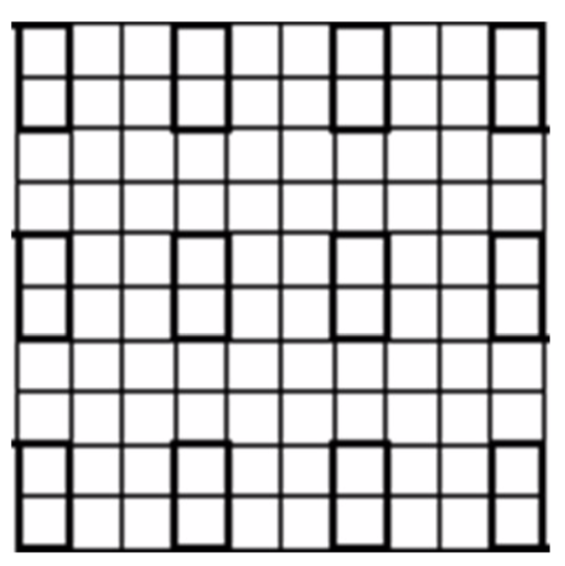
\includegraphics[width=0.20\textwidth]{PlaceForCruiser.png}%
%   \phantomsubcaption\label{fig:1c}% Bug: Produces an unwanted space
%   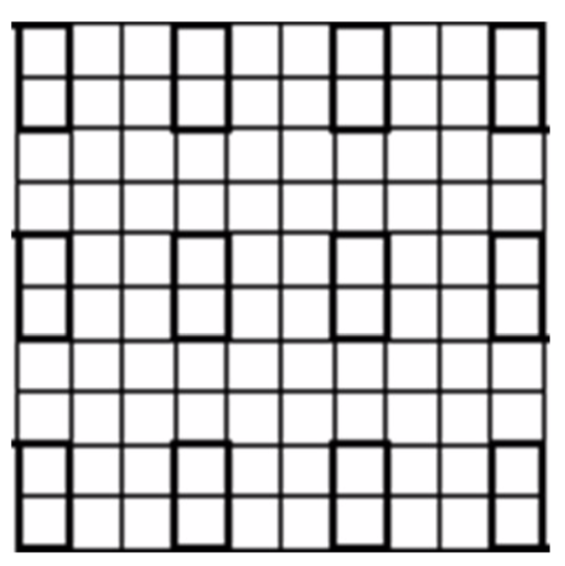
\includegraphics[width=0.20\textwidth]{PlaceForCruiser.png}%
%   \phantomsubcaption\label{fig:1d}%
%}
\captionbox{Grids for: \subref{fig:cruiser}: cruisers. \subref{fig:battleship}: battleships}{%
  \subcaptionbox{\label{fig:cruiser}}{%
    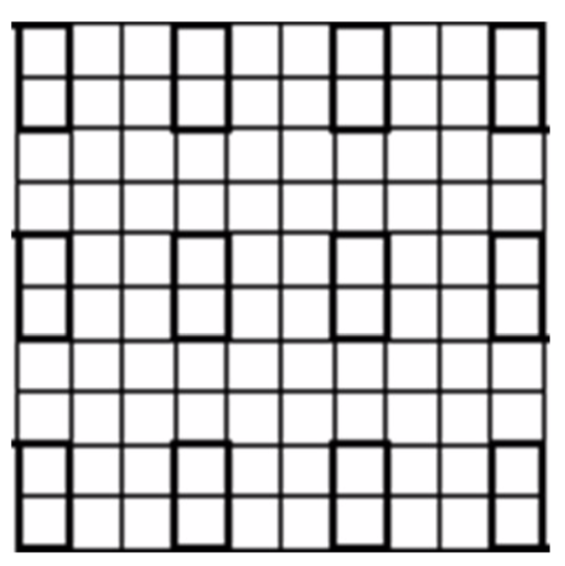
\includegraphics[width=0.20\textwidth]{PlaceForCruiser.png}}
  \subcaptionbox{\label{fig:battleship}}{%
    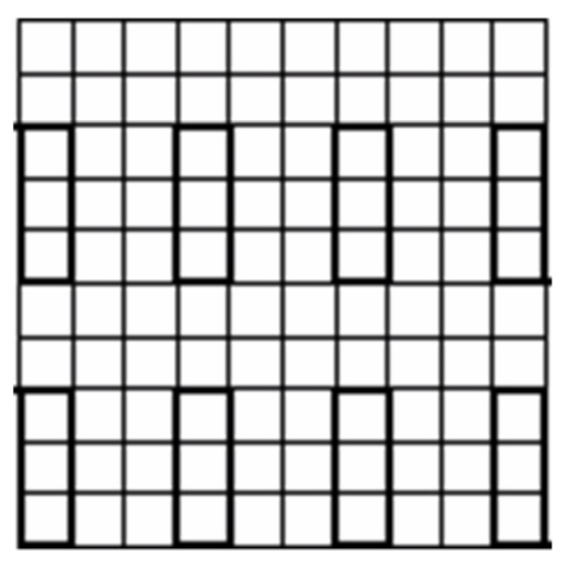
\includegraphics[width=0.20\textwidth]{PlaceForBattleship.png}}
}%
\end{center}
\end{figure}




\end{problem}
%

%2
\begin{problem}
\textit{[Elusive freedom of choice]}
Johnny had to choose $372$ distinct numbers out of set $\set{1,2,...,1200}$ with a property that no two chosen numbers have a difference of $4,5,$ or $9$. 

Prove that Johnny chose number $600$! 
\end{problem}
%

%%3
%\begin{problem}
%
%\textbf{Problem}
%
%\textit{[Very even tournament]}
%In a football tournament there are $n>4$ teams and every team has to play every other. Victory gives a team $3$ points, tie - $1$ point, loss - $0$ points. At the end of the tournament it happened that all the teams have equal number of points. 
%
%Prove that there exist $4$ teams, which have equal number of wins, ties and losses!
%
%\textbf{Solution}
%
%We group together teams with same number of wins, ties and losses. 
%
%Introduce notation, say, number of groups - $N$, and $v_i$, $l_i$, $t_i$ number of victories, losses, and ties for any team in group $i$, respectively. Since all teams have same number of points, then for any groups $i$ and $j$ the equality $3\times v_i+t_i=3\times v_j+t_j$ holds. From this follows (by simple number theory), that $t_i \equiv t_j$ mod $3$. On other hand, number of ties is limited by $0\le t_i \le n-1$ (team can tie with all others). 
%
%How many different numbers can be congruent to each other mod $3$ in the interval $[0,\dots, n-1]$? Well, if we split the $n$ numbers into groups of $3$ consecutive numbers - $[(0,1,2),(3,4,5),\dots]$ we will be able to take only one from each, so by PP we will have no more than $k=\ceil{\frac{n}{3}}=\floor{\frac{n+2}{3}}$.
%
%Therefore $N\le k$. Since $n>4$ then, by Pigeonhole, there will be at least one group with $3$ teams in it. 
%
%Let's assume the opposite of what we need to prove - that none of the groups have more than $3$ teams. Can it be that there are less than  $k$ groups? No, because $ (k-1) \times 3 = \floor{\frac{n+2}{3}} \times 3 - 3 < n$, therefore $N=k$. Designate the group with the smallest amount of ties $A$ and the group with largest amount of ties $B$.We have to consider three cases:
%\begin{enumerate}
%\item If $n=3k-2$, then
%\item If $n=3k-1$, then
%\item If $n=3k$, then
%\end{enumerate}
%
%\end{problem}
%

%4
\begin{problem}
\textit{[Convoluted treasure hunt]}
Miervaldis and Visvaldis are playing a following game. Large circle is drawn on an Euclidean field (plane). Miervaldis has hidden treasures in $n$ points within the circle. Visvaldis wishes to find all treasures.

One guess for Visvaldis is to choose a point on a field (within or without the circle) and Miervaldis announces distance from this point to the nearest unrecovered treasure or, if this distance is zero, uncovers the treasure. Visvaldis is capable of marking point in this plane, drawing straight lines and even using a (sufficiently large) compass.

Can Visvaldis find all the treasures with no more than $(n+1)^2$ guesses? 
\end{problem}
%

%5
\begin{problem}
\textit{[Splitting a square]}
Each of $9$ lines divide a square into two quadrilaterals, whose areas have a proportion of $2:3$ to each other. Prove that there exists a point, where at least three of these lines meet!
\end{problem}
%

%6
\begin{problem}
\textit{[Order out of randomness]}
Numbers $\set{1,2,3,...,101}$ are written in a line in some random order. Prove, that it is possible to erase $90$ of them so, that remaining $11$ are ordered in either ascending or descending order!
\end{problem}
%

%8
\begin{problem}
\textit{[Mindblowing triangles]}
Cells of an infinite grid are all colored in one of three colors each. Prove that it is possible to find a right triangle whose vertices are cells of the same color!
\end{problem}
%
\end{document}
